\section{介绍}

\begin{frame}
  \frametitle{介绍}

点云是一种重要的几何数据结构。由于其不规则的格式,大多数研究人员将这些数据转换为规则的3D体素网格或图像集合。然而,这使得数据不必要地庞大,并造成问题。研究人员设计了一种新型的神经网络PointNet,它直接以点云作为输入,考虑了输入点的排列不变性。PointNet提供了一个统一的架构,用于对象分类,物体分割,场景分割。

\begin{figure}
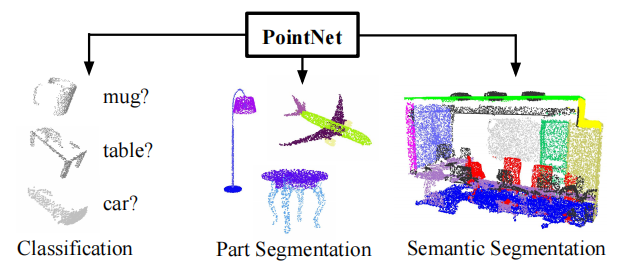
\includegraphics[scale=0.55]{doc/img/f1.png}
\caption{ 1}
\end{figure}

\end{frame}

\begin{frame}
 \frametitle{问题描述}

 研究者设计了一个深度学习框架,直接使用无序点集作为输入。点云表示为一组3D点 $\{P_i | i = 1, ... ,n \} $ ,其中每个点 $P_i$ 是其 $(x,y,z)$ 坐标加上诸如颜色、法线等的额外特征通道的向量。

对于对象分类任务,Pointnet为所有 $k$ 个候选类输出 $k$ 个分数。对于语义分割,输入可以是用于部分区域分割的单个对象,或者是用于对象区域分割的3D场景。Pointnet将为 $n$ 个点中的每个点生成 $m$ 个语义类别分数,共输出 $n \times m$ 个分数。

\end{frame}

\begin{frame}
\frametitle{相关工作}

\textbf{3D计算机视觉}

Volumetric CNNs:将三维卷积神经网络应用于体素化3D视觉学习。然而,由于3D数据的稀疏性和三维卷积的计算成本,体素表示受到其分辨率的限制。FPNN和Vote3D提出了处理稀疏性问题的特殊方法,然而,处理非常大的点云仍然是一个挑战。
Multiview CNNs:将三维点云渲染成二维图像,然后应用二维卷积网络对其进行分类。通过设计良好的图像学习网络,这种方法在形状分类和检索任务上取得了主要的性能。然而,将它们扩展到场景分割或其他3D任务,如点云补全是非常困难的。
Feature-based DNNs:将三维数据转换为一个向量,然后利用全连接网络对形状进行分类。这样提取到特征的表示能力有很大的约束,因为将无序的点云转化成了有序的向量。
    
\end{frame}

\begin{frame}
\frametitle{点云特性}
无序性,与图像中的像素阵列或体素网格中的体素阵列不同,点云是一组没有特定顺序的点,输入为N个点的网络需要对N!保持输出不变性。
交互性,点云中的这些点来自于具有相同距离度量的欧几里得空间。这意味着点与点之间不是孤立的,相邻的点形成了一个相互关联的子集,这意味着模型需要从附近的点捕获局部结构的语义特征。
仿射性,点云是一个完整的仿射对象,即对整个点云进行仿射变换如旋转和平移后仍和原始点云语义特征保持一致。
    
\end{frame}